\documentclass[a4paper,12pt]{extarticle}
\usepackage[utf8x]{inputenc}
\usepackage[T1,T2A]{fontenc}
\usepackage[russian]{babel}
\usepackage{hyperref}
\usepackage{indentfirst}
\usepackage{listings}
\usepackage{color}
\usepackage{here}
\usepackage{array}
\usepackage{multirow}
\usepackage{graphicx}
\usepackage{pgffor}

\usepackage{caption}
\renewcommand{\lstlistingname}{Программа} % заголовок листингов кода

\bibliographystyle{ugost2008ls}

\usepackage{listings}
\lstset{ %
extendedchars=\true,
keepspaces=true,
language=Matlab,						% choose the language of the code
basicstyle=\footnotesize,		% the size of the fonts that are used for the code
numbers=left,					% where to put the line-numbers
numberstyle=\footnotesize,		% the size of the fonts that are used for the line-numbers
stepnumber=1,					% the step between two line-numbers. If it is 1 each line will be numbered
numbersep=5pt,					% how far the line-numbers are from the code
backgroundcolor=\color{white},	% choose the background color. You must add \usepackage{color}
showspaces=false				% show spaces adding particular underscores
showstringspaces=false,			% underline spaces within strings
showtabs=false,					% show tabs within strings adding particular underscores
frame=single,           		% adds a frame around the code
tabsize=2,						% sets default tabsize to 2 spaces
captionpos=t,					% sets the caption-position to top
breaklines=true,				% sets automatic line breaking
breakatwhitespace=false,		% sets if automatic breaks should only happen at whitespace
escapeinside={\%*}{*)},			% if you want to add a comment within your code
postbreak=\raisebox{0ex}[0ex][0ex]{\ensuremath{\color{red}\hookrightarrow\space}},
texcl=true,
inputpath=listings,                     % директория с листингами
}

\usepackage[left=2cm,right=2cm,
top=2cm,bottom=2cm,bindingoffset=0cm]{geometry}

%% Нумерация картинок по секциям
\usepackage{chngcntr}
\counterwithin{figure}{section}
\counterwithin{table}{section}

%%Точки нумерации заголовков
\usepackage{titlesec}
\titlelabel{\thetitle.\quad}
\usepackage[dotinlabels]{titletoc}

%% Оформления подписи рисунка
\addto\captionsrussian{\renewcommand{\figurename}{Рисунок}}
\captionsetup[figure]{labelsep = period}

%% Подпись таблицы
\DeclareCaptionFormat{hfillstart}{\hfill#1#2#3\par}
\captionsetup[table]{format=hfillstart,labelsep=newline,justification=centering,skip=-10pt,textfont=bf}

%% Путь к каталогу с рисунками
\graphicspath{{fig/}}

%% Внесение titlepage в учёт счётчика страниц
\makeatletter
\renewenvironment{titlepage} {
 \thispagestyle{empty}
}
\makeatother


\begin{document}	% начало документа

% Титульная страница
\begin{titlepage}	% начало титульной страницы

	\begin{center}		% выравнивание по центру

		\large Санкт-Петербургский политехнический университет Петра Великого\\
		\large Институт компьютерных наук и технологий \\
		\large Кафедра компьютерных систем и программных технологий\\[6cm]
		% название института, затем отступ 6см
		
		\huge Вычислительная математика\\[0.5cm] % название работы, затем отступ 0,5см
		\large Отчет №1\\[0.1cm]
		\large Интерполяция функций\\[5cm]

	\end{center}


	\begin{flushright} % выравнивание по правому краю
		\begin{minipage}{0.25\textwidth} % врезка в половину ширины текста
			\begin{flushleft} % выровнять её содержимое по левому краю

				\large\textbf{Работу выполнил:}\\
				\large Граур А. А.\\
				\large {Группа:} 3530901/10006\\
				
				\large \textbf{Преподаватель:}\\
				\large Куляшова З. В.

			\end{flushleft}
		\end{minipage}
	\end{flushright}
	
	\vfill % заполнить всё доступное ниже пространство

	\begin{center}
	\large Санкт-Петербург\\
	\large \the\year % вывести дату
	\end{center} % закончить выравнивание по центру

\end{titlepage} % конец титульной страницы

\vfill % заполнить всё доступное ниже пространство


% Содержание
\include{ToC}

\section{Цель работы}
Ознакомление с интерполяцией/аппроксимацией функций, исследование погрешностей и работа с программным обеспечением MATLAB.

\section{Ход выполнения работы}

\subsection{Задача интерполяции Вандермонда}


\subsubsection{Задание}
Для \(y = sin(x)\) построить интерполяционные полиномы по точкам. Оценить и исследовать погрешность.
\begin{enumerate}
    \item Расширение границ интерполяции \([a, b]\): \([-\frac{\pi}{2};\frac{\pi}{2}]\);\([-\pi;\frac{\pi}{2}]\);\([-3\pi;3\pi]\)
    \item Увеличение количества точек (от 15 до 30)
    \item Добавление погрешности к заданным узлам интерполяции с помощью функции \(rand()\). (Уровни: 0.1, 0.01, 0.0001)
\end{enumerate}


\subsubsection{Границы \([-\frac{\pi}{2};\frac{\pi}{2}]\)}
Исследуем погрешность интерполяции на отрезке \([-\frac{\pi}{2};\frac{\pi}{2}]\).
\lstinputlisting[language=Matlab]{wandermond/first.m}
\begin{figure}[H]
\centering
    \foreach \n in {1,...,15}{
        \minipage{0.32\textwidth}
            \includegraphics[width=\linewidth]{wandermond/first/plot\n.png}
            \caption*{Погрешность для точки №\n}
        \endminipage\hfill
    }
\end{figure}
\begin{figure}
\centering
    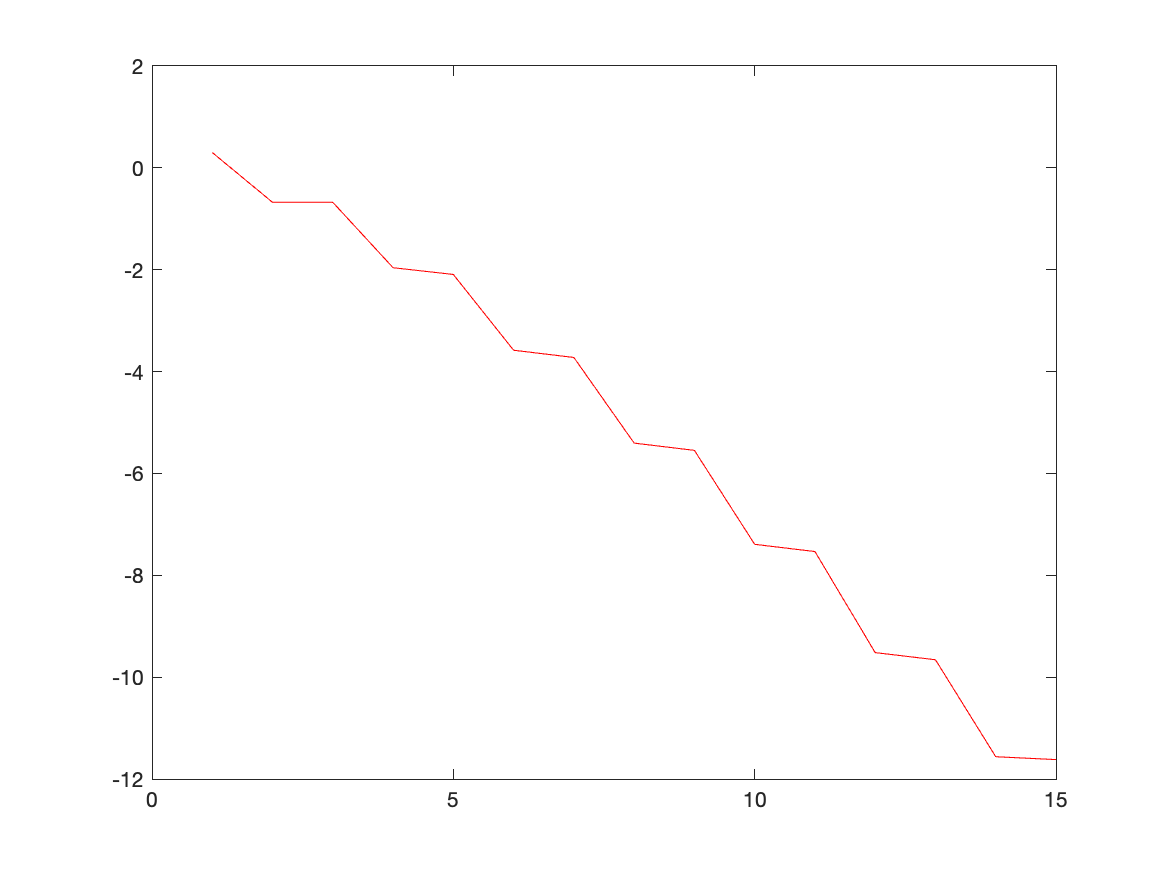
\includegraphics[scale=0.5]{wandermond/first/pogr.png}
    \caption{Общая погрешность}
\end{figure}


\subsubsection{Границы \([-\pi;\frac{\pi}{2}]\)}
Исследуем погрешность интерполяции на отрезке  \([-\pi;\frac{\pi}{2}]\).
\lstinputlisting[language=Matlab]{wandermond/second.m}
\begin{figure}[H]
    \centering
        \foreach \n in {1,...,15}{
            \minipage{0.32\textwidth}
                \includegraphics[width=\linewidth]{wandermond/second/plot\n.png}
                \caption*{Погрешность для точки №\n}
            \endminipage\hfill
        }
\end{figure}
\begin{figure}
\centering
    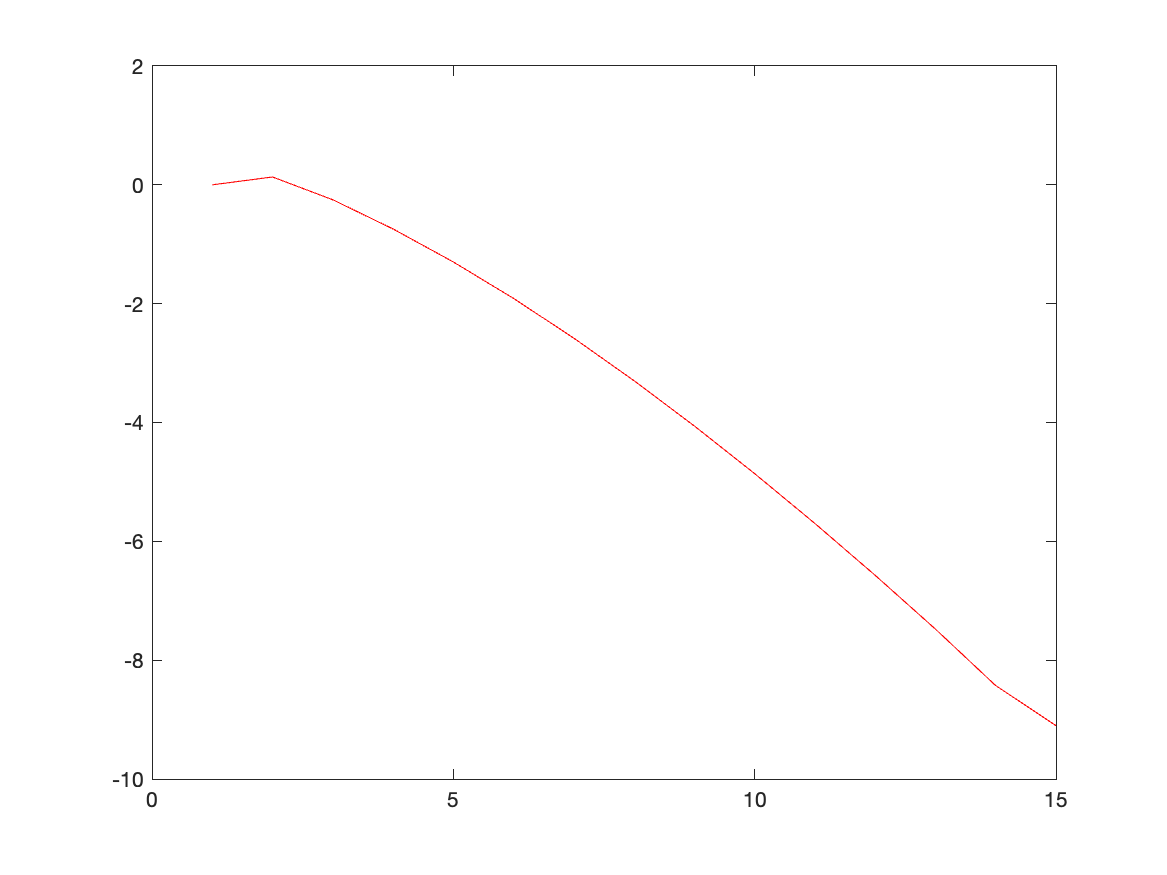
\includegraphics[scale=0.5]{wandermond/second/pogr.png}
    \caption{Общая погрешность}
\end{figure}


\subsubsection{Границы \([-3\pi;3\pi]\)}
Исследуем погрешность интерполяции на отрезке  \([-3\pi;3\pi]\).
\lstinputlisting[language=Matlab]{wandermond/third.m}
\begin{figure}[H]
    \centering
        \foreach \n in {1,...,15}{
            \minipage{0.32\textwidth}
                \includegraphics[width=\linewidth]{wandermond/third/plot\n.png}
                \caption*{Погрешность для точки №\n}
            \endminipage\hfill
        }
\end{figure}
\begin{figure}
\centering
    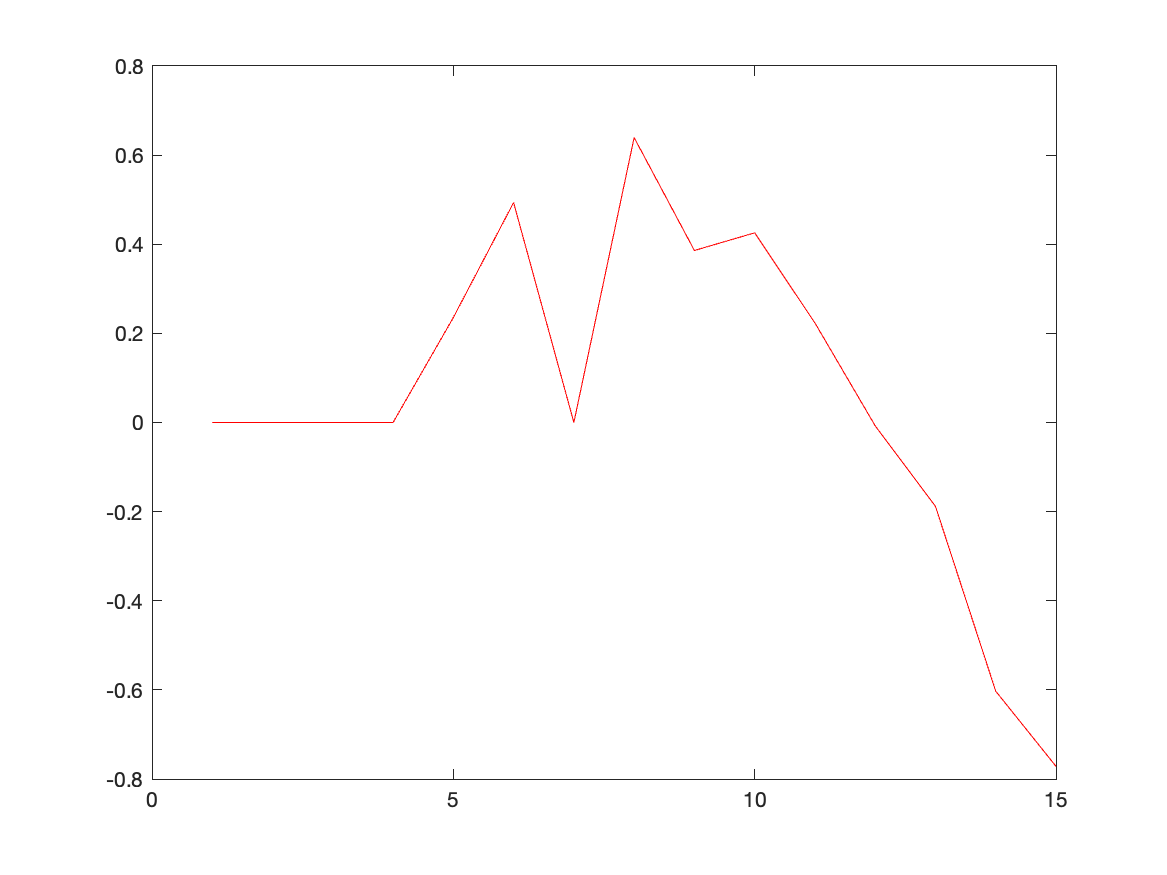
\includegraphics[scale=0.5]{wandermond/third/pogr.png}
    \caption{Общая погрешность}
\end{figure}

\textbf{Вывод по пунктам 2.1.2 - 2.1.4}: На полученных графиках для каждого интервала видно, что с каждой новой точкой интерполяции общая погрешность постепенно уменьшается.

\subsubsection{Увеличение количества точек до 30}
Исследуем погрешность интерполяции на отрезке  \([-3\pi;3\pi]\) с количеством точек \(m = 30\).
\lstinputlisting[language=Matlab]{wandermond/third_30.m}
\begin{figure}[H]
    \centering
        \foreach \n in {1,...,15}{
            \minipage{0.32\textwidth}
                \includegraphics[width=\linewidth]{wandermond/third_30/plot\n.png}
                \caption*{Погрешность для точки №\n}
            \endminipage\hfill
        }
\end{figure}
\begin{figure}[H]
    \centering
        \foreach \n in {16,...,30}{
            \minipage{0.32\textwidth}
                \includegraphics[width=\linewidth]{wandermond/third_30/plot\n.png}
                \caption*{Погрешность для точки №\n}
            \endminipage\hfill
        }
\end{figure}
\begin{figure}
\centering
    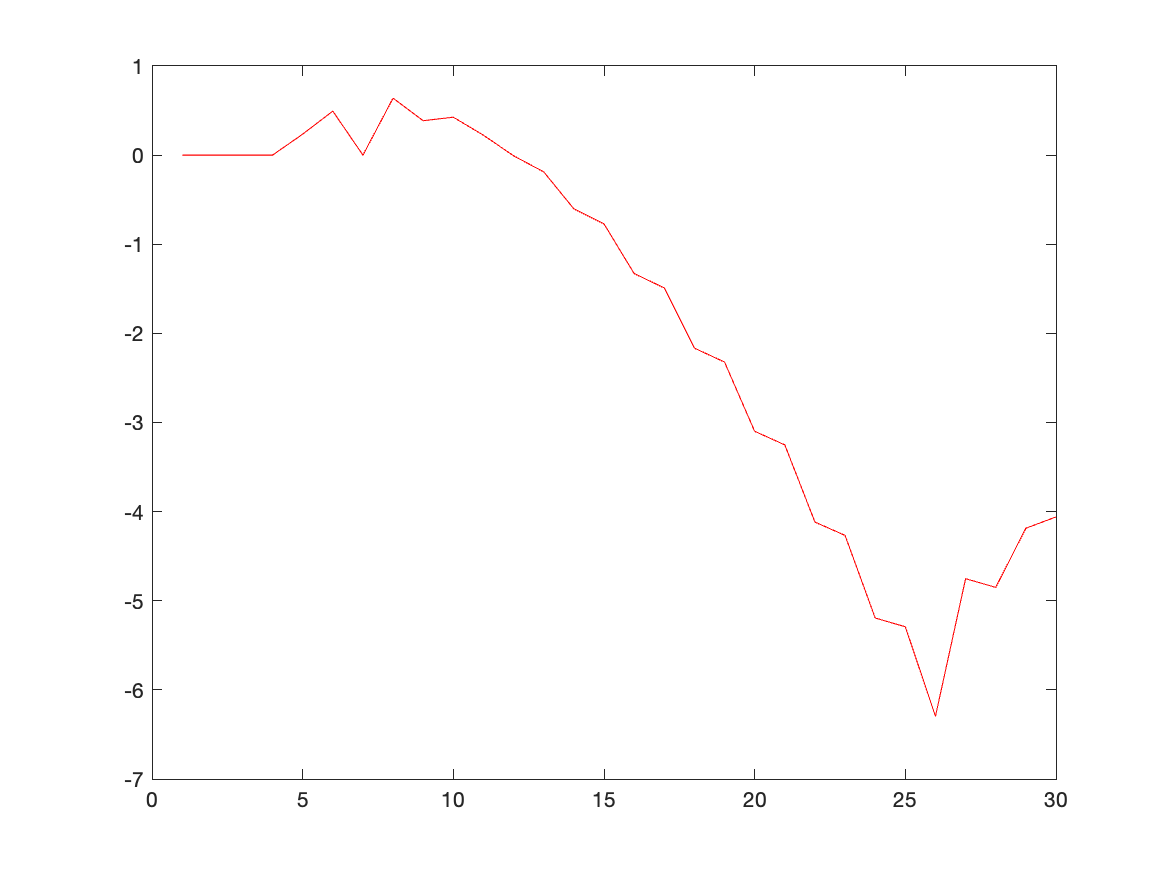
\includegraphics[scale=0.5]{wandermond/third_30/pogr.png}
    \caption{Общая погрешность}
\end{figure}

\textbf{Вывод:} По полученным графикам можно заметить, что после 15-й точки интерполяции погрешность начинает, наоборот возрастать.

\subsubsection{Добавление погрешности. Уровень 0.1}
Исследуем погрешность интерполяции на отрезке  \([-3\pi;3\pi]\) с количеством точек \(m = 30\) и с добавлением погрешности уровня 0.1
\lstinputlisting[language=Matlab]{wandermond/third_01.m}
\begin{figure}[H]
    \centering
        \foreach \n in {1,...,15}{
            \minipage{0.32\textwidth}
                \includegraphics[width=\linewidth]{wandermond/third_01/plot\n.png}
                \caption*{Погрешность для точки №\n}
            \endminipage\hfill
        }
\end{figure}
\begin{figure}[H]
    \centering
        \foreach \n in {16,...,30}{
            \minipage{0.32\textwidth}
                \includegraphics[width=\linewidth]{wandermond/third_01/plot\n.png}
                \caption*{Погрешность для точки №\n}
            \endminipage\hfill
        }
\end{figure}
\begin{figure}
\centering
    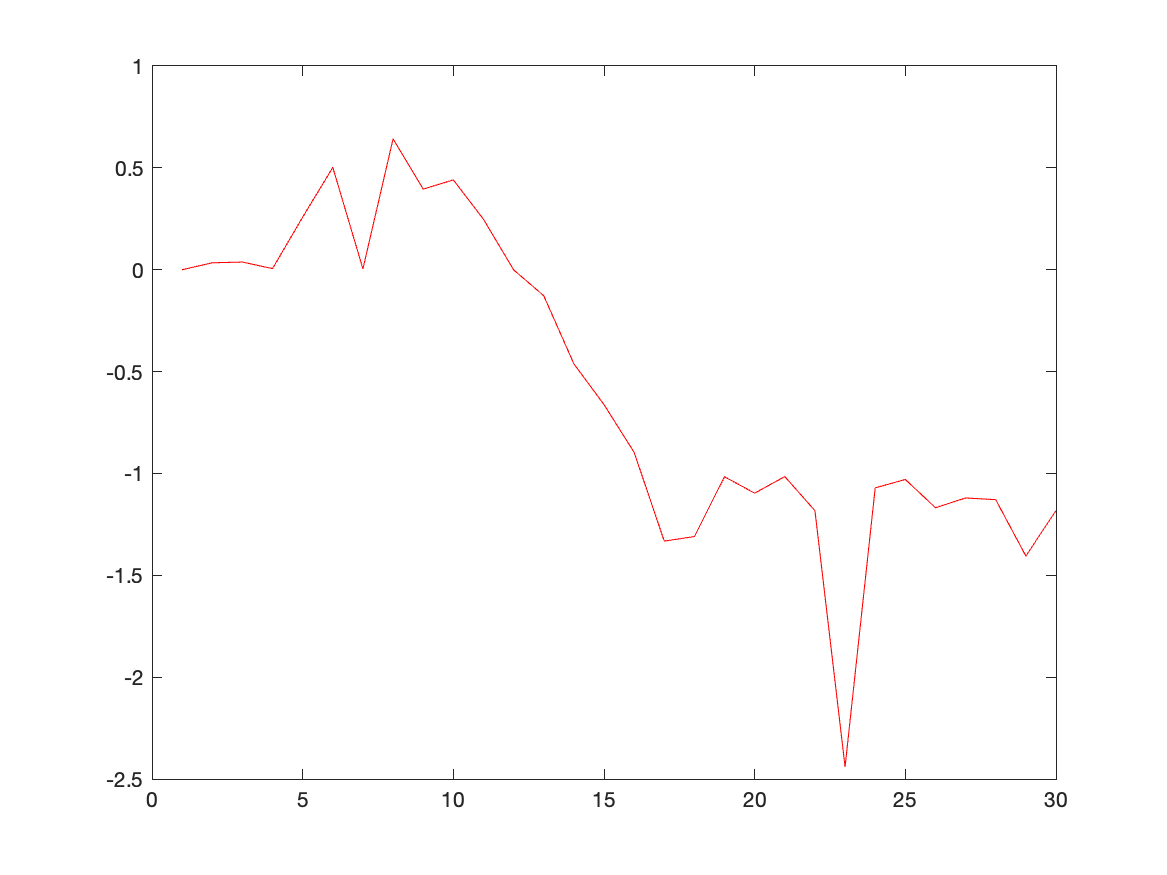
\includegraphics[scale=0.5]{wandermond/third_01/pogr.png}
    \caption{Общая погрешность}
\end{figure}


\subsubsection{Добавление погрешности. Уровень 0.01}
Исследуем погрешность интерполяции на отрезке  \([-3\pi;3\pi]\) с количеством точек \(m = 30\) и с добавлением погрешности уровня 0.01
\lstinputlisting[language=Matlab]{wandermond/third_001.m}
\begin{figure}[H]
    \centering
        \foreach \n in {1,...,15}{
            \minipage{0.32\textwidth}
                \includegraphics[width=\linewidth]{wandermond/third_001/plot\n.png}
                \caption*{Погрешность для точки №\n}
            \endminipage\hfill
        }
\end{figure}
\begin{figure}[H]
    \centering
        \foreach \n in {16,...,30}{
            \minipage{0.32\textwidth}
                \includegraphics[width=\linewidth]{wandermond/third_001/plot\n.png}
                \caption*{Погрешность для точки №\n}
            \endminipage\hfill
        }
\end{figure}
\begin{figure}
\centering
    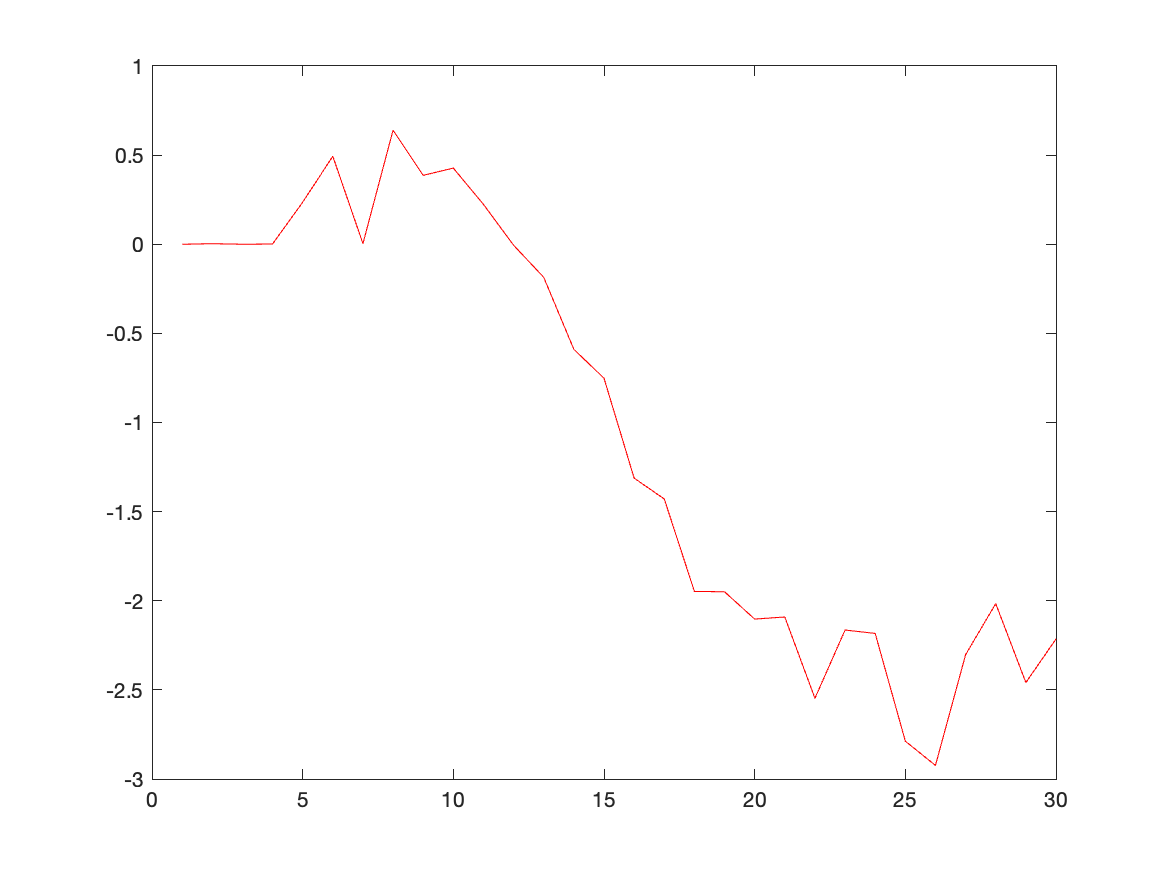
\includegraphics[scale=0.5]{wandermond/third_001/pogr.png}
    \caption{Общая погрешность}
\end{figure}

\subsubsection{Добавление погрешности. Уровень 0.0001}
Исследуем погрешность интерполяции на отрезке  \([-3\pi;3\pi]\) с количеством точек \(m = 30\) и с добавлением погрешности уровня 0.0001
\lstinputlisting[language=Matlab]{wandermond/third_00001.m}
\begin{figure}[H]
    \centering
        \foreach \n in {1,...,15}{
            \minipage{0.32\textwidth}
                \includegraphics[width=\linewidth]{wandermond/third_00001/plot\n.png}
                \caption*{Погрешность для точки №\n}
            \endminipage\hfill
        }
\end{figure}
\begin{figure}[H]
    \centering
        \foreach \n in {16,...,30}{
            \minipage{0.32\textwidth}
                \includegraphics[width=\linewidth]{wandermond/third_00001/plot\n.png}
                \caption*{Погрешность для точки №\n}
            \endminipage\hfill
        }
\end{figure}
\begin{figure}
\centering
    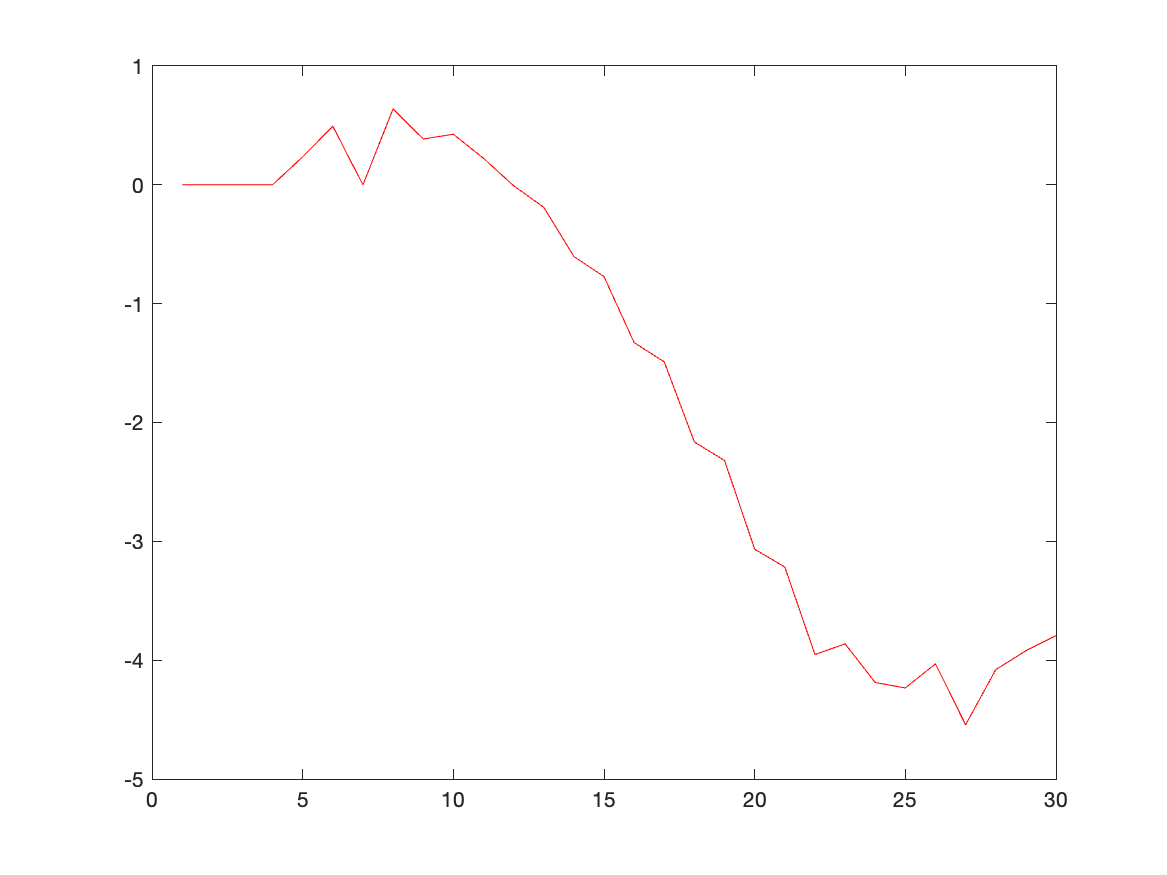
\includegraphics[scale=0.5]{wandermond/third_00001/pogr.png}
    \caption{Общая погрешность}
\end{figure}

\textbf{Вывод по пунктам 2.1.6-2.1.8:} По полученным графикам, видно, что добавление погрешности \(rand()\) придаёт хаотичность графикам погрешностей.


\subsection{Интерполяционный полином Ньютона и Лагранжа}
\begin{center}
Формула интерполяционного полинома в форме Ньютона
\[P_n(x)=f(x_0)+(x-x_0)f(x_0;x_1)+(x-x_0)(x-x_1)f(x_0;x_1;x_2)+\cdots+(x-x_{n-1})f(x_0;\cdots;x_n)\]
Функция для вычисления интерполяционного полинома в форме Ньютона
\lstinputlisting[language=Matlab]{newton/newton.m}
Формула интерполяционного полинома в форме Лагранжа
\[L_n(x)=\sum_{k=1}^{n+1} y_k \prod_{j=1,2,...n+1,j\not=k}\frac{x-x_j}{x_k-x_j}\]
Функция для вычисления интерполяционного полинома в форме Лагранжа
\lstinputlisting[language=Matlab]{lagrange/lagrange.m}
Проверим работу функций, для чего создадим отдельный файл script.m
\lstinputlisting[language=Matlab]{newton/script.m}
\begin{figure}[H]
\minipage{0.5\textwidth}
    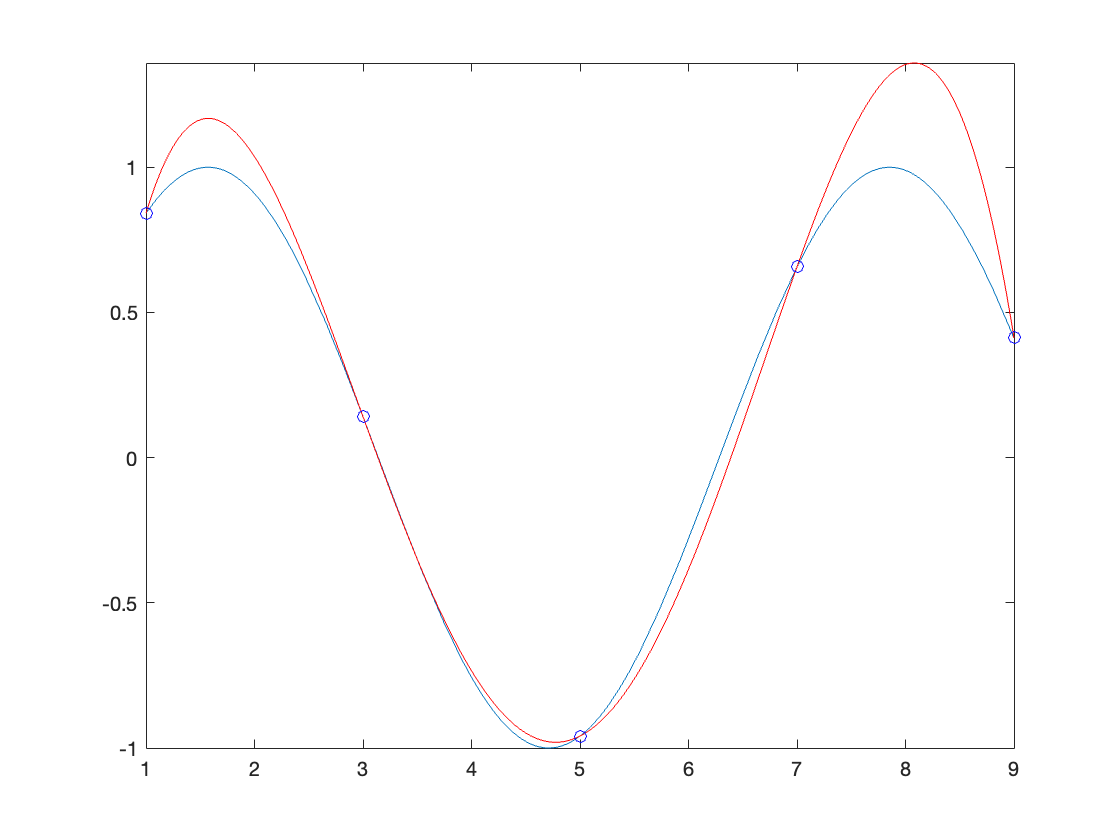
\includegraphics[width=\linewidth]{newton.png}
    \caption*{График полинома в форме Ньютона}
\endminipage\hfill
\minipage{0.5\textwidth}
    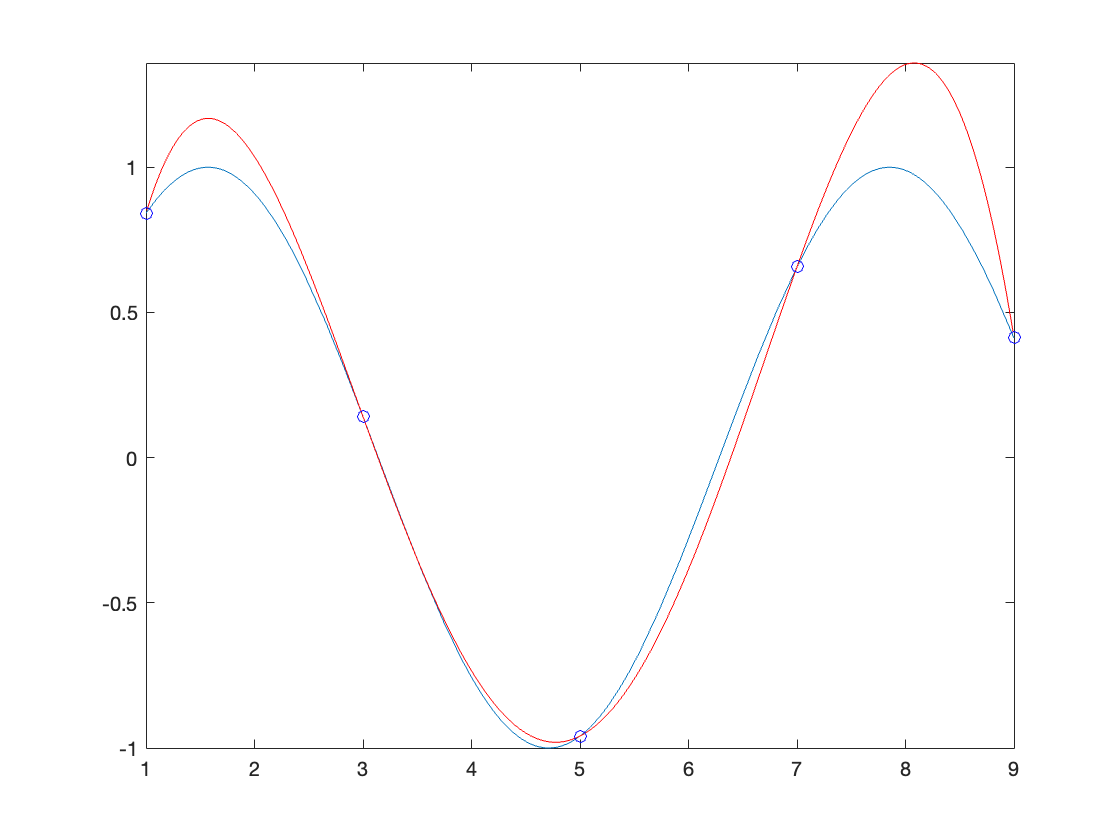
\includegraphics[width=\linewidth]{lagrange.png}
    \caption*{График полинома в форме Лагранжа}
\endminipage\hfill
\end{figure}
\end{center}
\textbf{Вывод:} По полученным графикам можно подтвердить тот факт, что полином Лагранжа равен полиному Ньютона.


\subsection{Минимизация погрешности интерполяции по Чебышеву}
При интерполировании функции полиномами Лагранжа или Ньютона возникает погрешность, которую можно минимизировать с помощью интерполяции по Чебышеву.

Для натурального числа n узлы Чебышёва на отрезке [−1, 1] задаются формулой
\[T_k=\cos{\frac{2k-1}{2n}\pi}\]
Это корни многочлена Чебышёва первого рода степени n. Для получения узлов на произвольном отрезке [a, b] можно применить аффинное преобразование отрезков:
\[x_k=\frac{a+b}{2}+\frac{b-a}{2}T_k\]
\lstinputlisting[language=Matlab]{chebyshev.m}
\begin{figure}[H]
    \centering
        \foreach \n in {1,...,10}{
            \minipage{0.3\textwidth}
                \includegraphics[width=\linewidth]{chebyshev/plot\n.png}
                \caption*{Погрешность для точки №\n}
            \endminipage\hfill
        }
        \minipage{0.3\textwidth}
            \includegraphics*[width=\linewidth]{chebyshev/dp.png}
            \caption*{Общая погрешность}
        \endminipage\hfill
\end{figure}
\textbf{Вывод:} При анализе полученных графиков, можно заметить, что при интерполяции по Чебышеву погрешность действительно меньше.

\subsection{Интерполяция сплайнами}
\textbf{Сплайн} — функция в математике, область определения которой разбита на конечное число отрезков, на каждом из которых она совпадает с некоторым алгебраическим многочленом (полиномом).

Другими словами сплайн — это кусочно заданная функция, то есть совокупность нескольких функций, каждая из которых задана на каком-то множестве значений аргумента, причём эти множества попарно непересекающиеся.

\lstinputlisting[language=Matlab]{splines.m}
На рисунке представлены погрешность интерполирования для полинома с \textcolor{blue}{равномерно расставленными узлами}, \textcolor{red}{узлами Чебышева} и \textcolor{green}{сплайнами}
\begin{figure}[H]
    \centering
    \minipage{0.32\textwidth}
        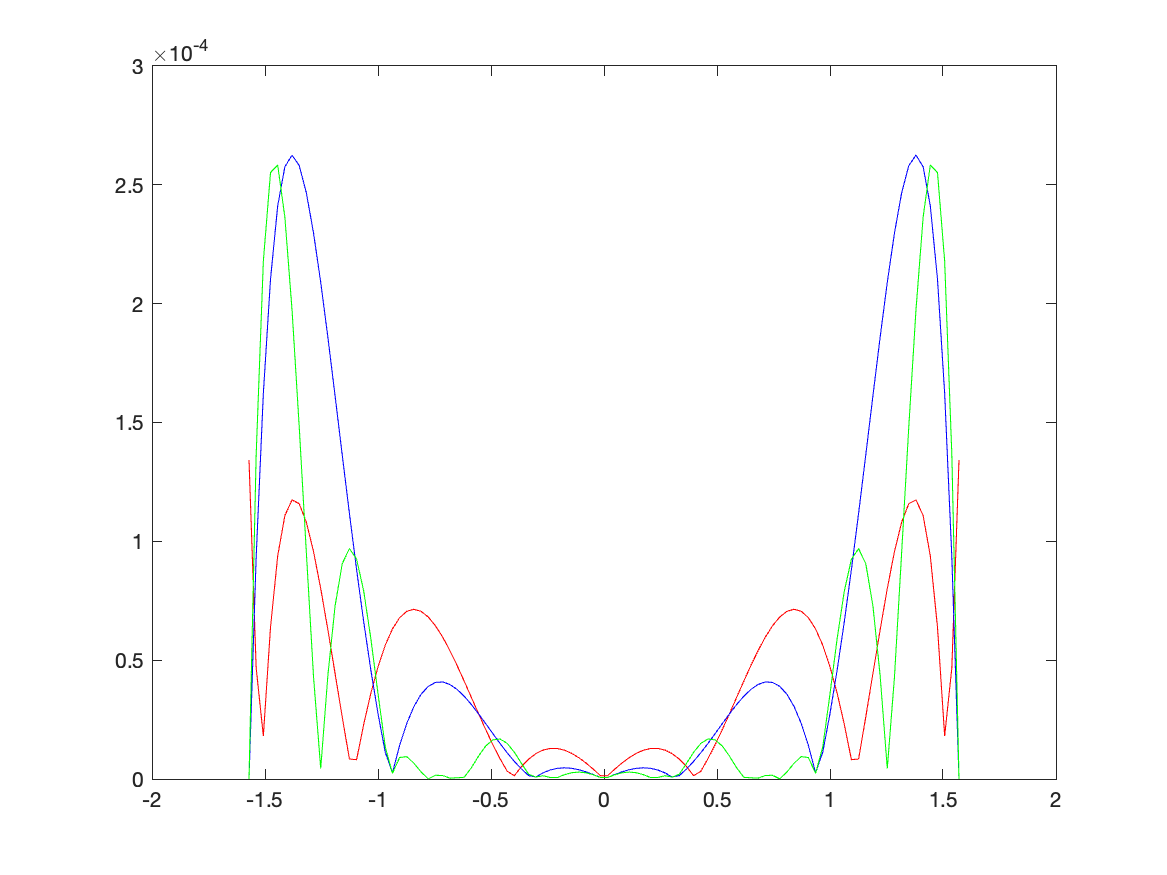
\includegraphics[width=\linewidth]{splines/spline_5_10.png}
        \caption*{m = 5, n = 10}
    \endminipage\hfill
    \minipage{0.32\textwidth}
        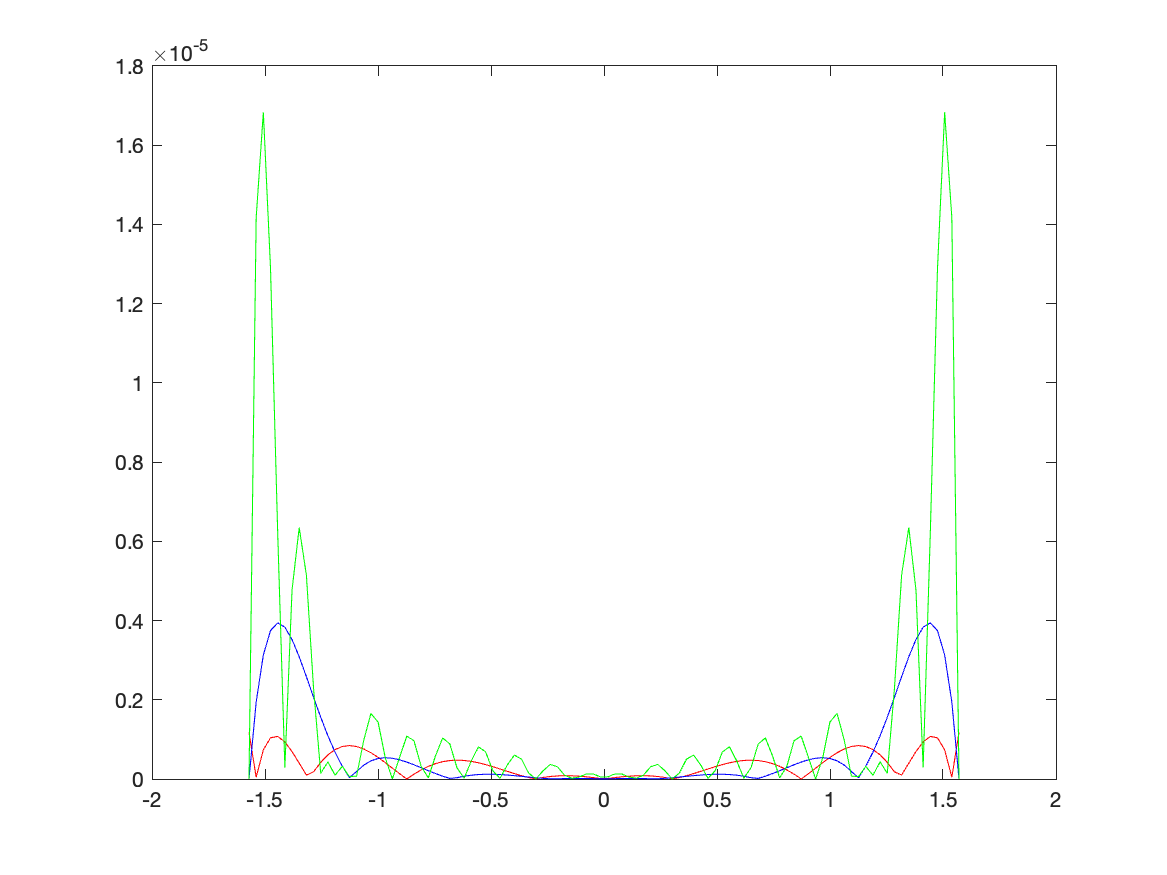
\includegraphics[width=\linewidth]{splines/spline_7_20.png}
        \caption*{m = 7, n = 20}
    \endminipage\hfill
    \minipage{0.32\textwidth}
        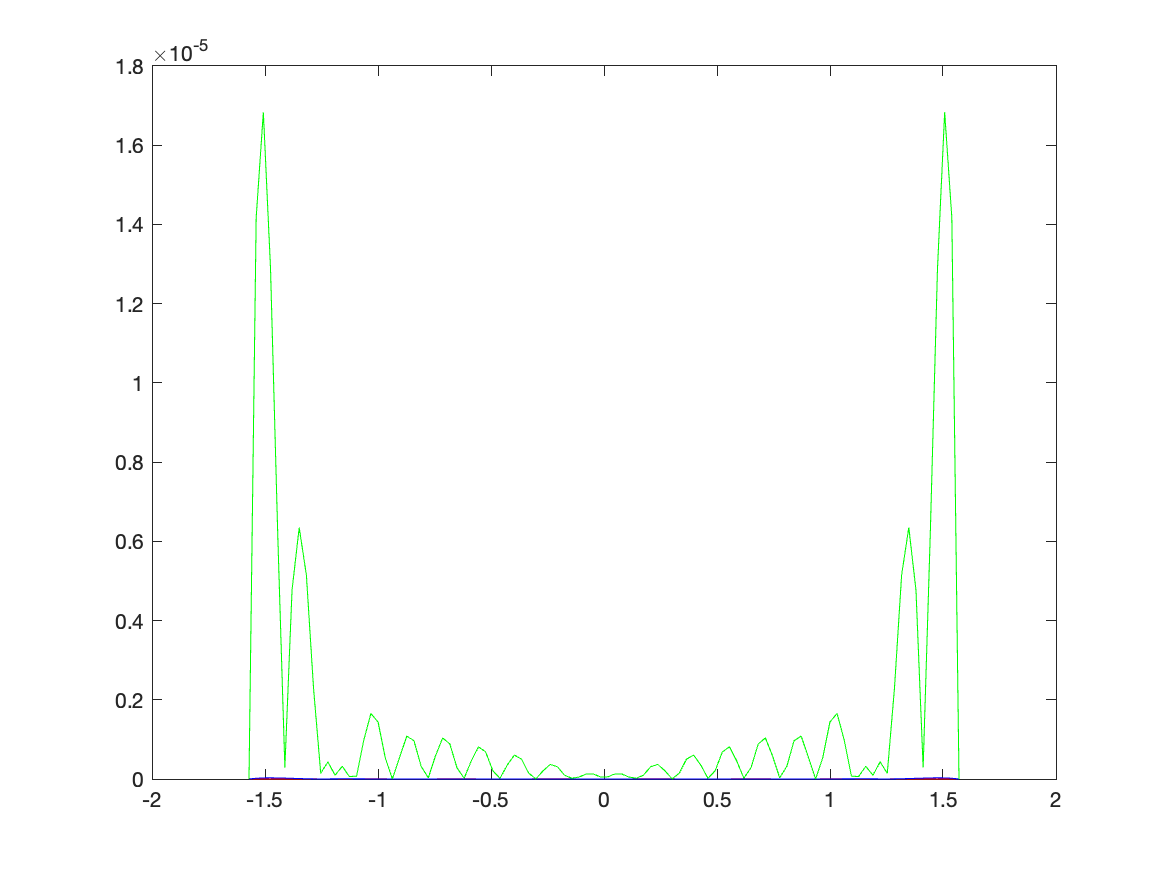
\includegraphics[width=\linewidth]{splines/spline_10_20.png}
        \caption*{m = 10, n = 20}
    \endminipage\hfill
    \minipage{0.32\textwidth}
        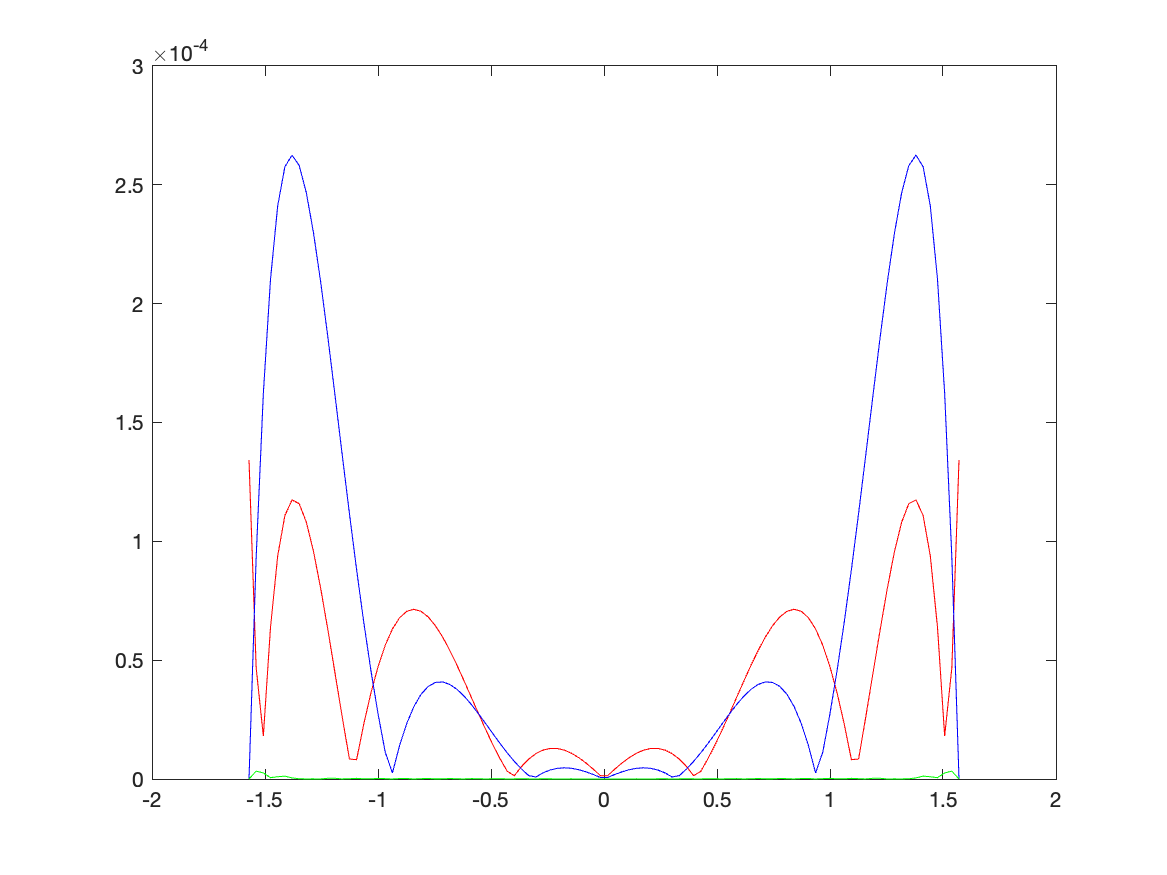
\includegraphics[width=\linewidth]{splines/spline_5_30.png}
        \caption*{m = 5, n = 30}
    \endminipage\hfill
    \minipage{0.32\textwidth}
        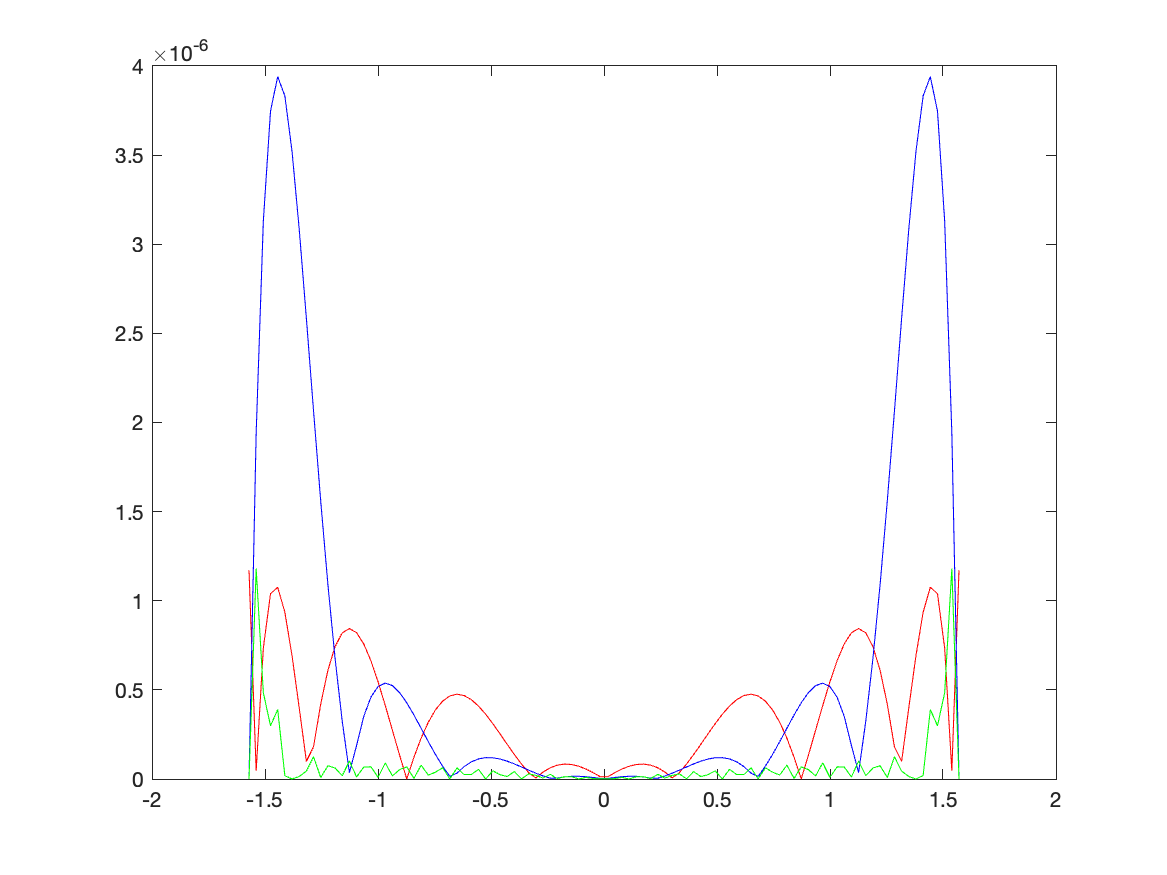
\includegraphics[width=\linewidth]{splines/spline_7_39.png}
        \caption*{m = 7, n = 39}
    \endminipage\hfill
    \minipage{0.32\textwidth}
        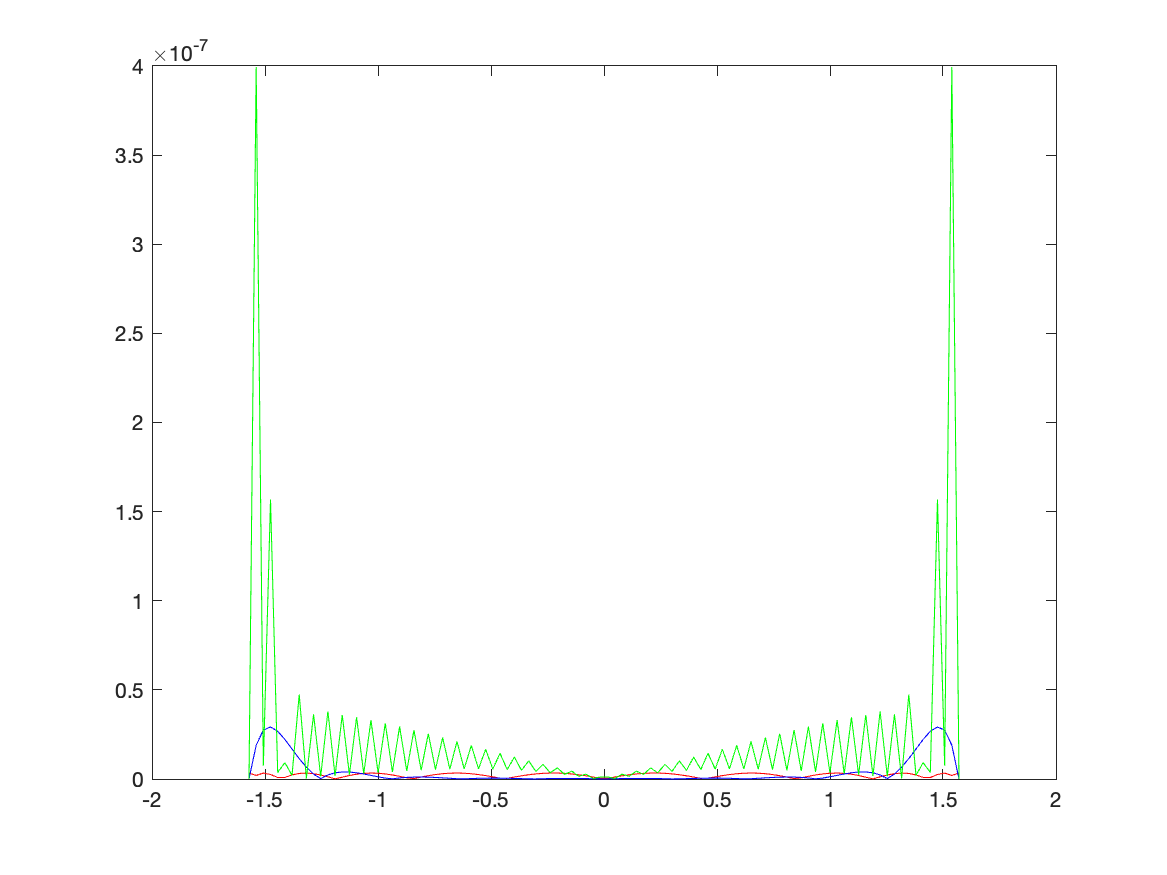
\includegraphics[width=\linewidth]{splines/spline_10_50.png}
        \caption*{m = 10, n = 50}
    \endminipage\hfill
\end{figure}
\textbf{Вывод:} При уменьшении количества узлов и увелечении количества отрезков сплайна, интерполирование сплайнами становится эффективнее.
\end{document}
